%%%%%%%%%%%%%%%%%%%%%%%%%%%%%%%%%%%%%%%%%
% Lachaise Assignment
% LaTeX Template
% Version 1.0 (26/6/2018)
%
% This template originates from:
% http://www.LaTeXTemplates.com
%
% Authors:
% Marion Lachaise & François Févotte
% Vel (vel@LaTeXTemplates.com)
%
% License:
% CC BY-NC-SA 3.0 (http://creativecommons.org/licenses/by-nc-sa/3.0/)
%
%%%%%%%%%%%%%%%%%%%%%%%%%%%%%%%%%%%%%%%%%

%----------------------------------------------------------------------------------------
%	PACKAGES AND OTHER DOCUMENT CONFIGURATIONS
%----------------------------------------------------------------------------------------

\documentclass{article}

%%%%%%%%%%%%%%%%%%%%%%%%%%%%%%%%%%%%%%%%%
% Lachaise Assignment
% Structure Specification File
% Version 1.0 (26/6/2018)
%
% This template originates from:
% http://www.LaTeXTemplates.com
%
% Authors:
% Marion Lachaise & François Févotte
% Vel (vel@LaTeXTemplates.com)
%
% License:
% CC BY-NC-SA 3.0 (http://creativecommons.org/licenses/by-nc-sa/3.0/)
%
%%%%%%%%%%%%%%%%%%%%%%%%%%%%%%%%%%%%%%%%%

%----------------------------------------------------------------------------------------
%	PACKAGES AND OTHER DOCUMENT CONFIGURATIONS
%----------------------------------------------------------------------------------------

\usepackage{amsmath,amsfonts,stmaryrd,amssymb} % Math packages

\usepackage{enumerate} % Custom item numbers for enumerations

\usepackage[ruled]{algorithm2e} % Algorithms

\usepackage[framemethod=tikz]{mdframed} % Allows defining custom boxed/framed environments

\usepackage{listings} % File listings, with syntax highlighting

\usepackage{color} %red, green, blue, yellow, cyan, magenta, black, white
\definecolor{mygreen}{RGB}{28,172,0} % color values Red, Green, Blue
\definecolor{mylilas}{RGB}{170,55,241}
\usepackage{float}
\usepackage{amsmath}% http://ctan.org/pkg/amsmath
\newcommand\Inn{%
  \mathrel{\ooalign{$\subset$\cr\hfil\scalebox{0.8}[1]{$=$}\hfil\cr}}%
}
% \mathcode`*=\string"8000

\lstset{
	basicstyle=\ttfamily, % Typeset listings in monospace font
}


% matlab desciption
% usage \lstinputlisting{/path/to/matlab/code.m}

\lstset{language=Matlab,%
    %basicstyle=\color{red},
    breaklines=true,%
    morekeywords={matlab2tikz},
    keywordstyle=\color{blue},%
    morekeywords=[2]{1}, keywordstyle=[2]{\color{black}},
    identifierstyle=\color{black},%
    stringstyle=\color{mylilas},
    commentstyle=\color{mygreen},%
    showstringspaces=false,%without this there will be a symbol in the places where there is a space
    numbers=none,%
    numberstyle={\tiny \color{black}},% size of the numbers
    numbersep=9pt, % this defines how far the numbers are from the text
    emph=[1]{for,end,break},emphstyle=[1]\color{red}, %some words to emphasise
    %emph=[2]{word1,word2}, emphstyle=[2]{style},
}


%----------------------------------------------------------------------------------------
%	DOCUMENT MARGINS
%----------------------------------------------------------------------------------------

\usepackage{geometry} % Required for adjusting page dimensions and margins

\geometry{
	paper=a4paper, % Paper size, change to letterpaper for US letter size
	top=2.5cm, % Top margin
	bottom=3cm, % Bottom margin
	left=2.5cm, % Left margin
	right=2.5cm, % Right margin
	headheight=14pt, % Header height
	footskip=1.5cm, % Space from the bottom margin to the baseline of the footer
	headsep=1.2cm, % Space from the top margin to the baseline of the header
	%showframe, % Uncomment to show how the type block is set on the page
}

%----------------------------------------------------------------------------------------
%	FONTS
%----------------------------------------------------------------------------------------

\usepackage[utf8]{inputenc} % Required for inputting international characters
\usepackage[T1]{fontenc} % Output font encoding for international characters

\usepackage{XCharter} % Use the XCharter fonts

%----------------------------------------------------------------------------------------
%	COMMAND LINE ENVIRONMENT
%----------------------------------------------------------------------------------------

% Usage:
% \begin{commandline}
%	\begin{verbatim}
%		$ ls
%
%		Applications	Desktop	...
%	\end{verbatim}
% \end{commandline}

\mdfdefinestyle{commandline}{
	leftmargin=10pt,
	rightmargin=10pt,
	innerleftmargin=15pt,
	middlelinecolor=black!50!white,
	middlelinewidth=2pt,
	frametitlerule=false,
	backgroundcolor=black!5!white,
	frametitle={Command Line},
	frametitlefont={\normalfont\sffamily\color{white}\hspace{-1em}},
	frametitlebackgroundcolor=black!50!white,
	nobreak,
}

% Define a custom environment for command-line snapshots
\newenvironment{commandline}{
	\medskip
	\begin{mdframed}[style=commandline]
}{
	\end{mdframed}
	\medskip
}

%----------------------------------------------------------------------------------------
%	FILE CONTENTS ENVIRONMENT
%----------------------------------------------------------------------------------------

% Usage:
% \begin{file}[optional filename, defaults to "File"]
%	File contents, for example, with a listings environment
% \end{file}

\mdfdefinestyle{file}{
	innertopmargin=1.6\baselineskip,
	innerbottommargin=0.8\baselineskip,
	topline=false, bottomline=false,
	leftline=false, rightline=false,
	leftmargin=2cm,
	rightmargin=2cm,
	singleextra={%
		\draw[fill=black!10!white](P)++(0,-1.2em)rectangle(P-|O);
		\node[anchor=north west]
		at(P-|O){\ttfamily\mdfilename};
		%
		\def\l{3em}
		\draw(O-|P)++(-\l,0)--++(\l,\l)--(P)--(P-|O)--(O)--cycle;
		\draw(O-|P)++(-\l,0)--++(0,\l)--++(\l,0);
	},
	nobreak,
}

% Define a custom environment for file contents
\newenvironment{file}[1][File]{ % Set the default filename to "File"
	\medskip
	\newcommand{\mdfilename}{#1}
	\begin{mdframed}[style=file]
}{
	\end{mdframed}
	\medskip
}

%----------------------------------------------------------------------------------------
%	NUMBERED QUESTIONS ENVIRONMENT
%----------------------------------------------------------------------------------------

% Usage:
% \begin{question}[optional title]
%	Question contents
% \end{question}

\mdfdefinestyle{question}{
	innertopmargin=1.2\baselineskip,
	innerbottommargin=0.8\baselineskip,
	roundcorner=5pt,
	nobreak,
	singleextra={%
		\draw(P-|O)node[xshift=1em,anchor=west,fill=white,draw,rounded corners=5pt]{%
		Question \theQuestion\questionTitle};
	},
}

\newcounter{Question} % Stores the current question number that gets iterated with each new question

% Define a custom environment for numbered questions
\newenvironment{question}[1][\unskip]{
	\bigskip
	\stepcounter{Question}
	\newcommand{\questionTitle}{~#1}
	\begin{mdframed}[style=question]
}{
	\end{mdframed}
	\medskip
}

%----------------------------------------------------------------------------------------
%	WARNING TEXT ENVIRONMENT
%----------------------------------------------------------------------------------------

% Usage:
% \begin{warn}[optional title, defaults to "Warning:"]
%	Contents
% \end{warn}

\mdfdefinestyle{warning}{
	topline=false, bottomline=false,
	leftline=false, rightline=false,
	nobreak,
	singleextra={%
		\draw(P-|O)++(-0.5em,0)node(tmp1){};
		\draw(P-|O)++(0.5em,0)node(tmp2){};
		\fill[black,rotate around={45:(P-|O)}](tmp1)rectangle(tmp2);
		\node at(P-|O){\color{white}\scriptsize\bf !};
		\draw[very thick](P-|O)++(0,-1em)--(O);%--(O-|P);
	}
}

% Define a custom environment for warning text
\newenvironment{warn}[1][Warning:]{ % Set the default warning to "Warning:"
	\medskip
	\begin{mdframed}[style=warning]
		\noindent{\textbf{#1}}
}{
	\end{mdframed}
}

%----------------------------------------------------------------------------------------
%	INFORMATION ENVIRONMENT
%----------------------------------------------------------------------------------------

% Usage:
% \begin{info}[optional title, defaults to "Info:"]
% 	contents
% 	\end{info}

\mdfdefinestyle{info}{%
	topline=false, bottomline=false,
	leftline=false, rightline=false,
	nobreak,
	singleextra={%
		\fill[black](P-|O)circle[radius=0.4em];
		\node at(P-|O){\color{white}\scriptsize\bf i};
		\draw[very thick](P-|O)++(0,-0.8em)--(O);%--(O-|P);
	}
}

% Define a custom environment for information
\newenvironment{info}[1][Info:]{ % Set the default title to "Info:"
	\medskip
	\begin{mdframed}[style=info]
		\noindent{\textbf{#1}}
}{
	\end{mdframed}
}
 % Include the file specifying the document structure and custom commands
\usepackage{graphicx}
\newcommand{\ts}{\textsuperscript}
\usepackage{float}


%----------------------------------------------------------------------------------------
%	ASSIGNMENT INFORMATION
%----------------------------------------------------------------------------------------

\title{Computational Engineering - Engr 8103 \\ Problem Set \#3} % Title of the assignment

\author{Allen Spain\\ \texttt{avs81684@uga.edu}} % Author name and email address

\date{University of Georgia --- 09 December 2019 } % University, school and/or department name(s) and a date

%----------------------------------------------------------------------------------------

\begin{document}

\maketitle % Print the title

%----------------------------------------------------------------------------------------
%	INTRODUCTION
%----------------------------------------------------------------------------------------

\section*{Question 1} % Unnumbered section
(5 pts.) Do this exercise with paper and pen, without using Matlab. Carry out the first four Newton iterations to find the root of $f(x) = x^{3} - 2x + 2$ with an initial guess of $x_{0} = 0$. Does it work? Explain the problem by sketching the graph of the function and the tangents.

% ----------------
% Answer goes here
% ----------------
\noindent
Give Newton's Method $x_{n+1} = x_{n} - \frac{f(x_{n})}{f^{\prime}(x_{n})}$, where $n$ is the iteration

\begin{tabular} {l | c |  r}
  $ n $ & $x_{n}$ & $x_{n+1}$\\
  $ 0 $& $ 0 $ & $x_{1} =  0 - \frac{[(0)^3 - 2(0) + 2]}{3(0)^{2} - 2} = 0 - \frac{-2}{-2} = 1$\\
  $ 1 $ & $ 1 $ & $x_{2} =  1 - \frac{[(1)^3 - 2(1) + 2]}{3(1)^{2} - 2} = 1 - \frac{1}{1} = 0$\\
  $ 2 $ & $ 0 $ & $x_{3} =  0 - \frac{[(0)^3 - 2(0) + 2]}{3(0)^{2} - 2} = 0 - \frac{-2}{-2} = 1$\\
  $ 3 $ & $ 1 $ & $x_{4} =  1 - \frac{[(1)^3 - 2(1) + 2]}{3(1)^{2} - 2} = 1 - \frac{1}{1} = 0$
\end{tabular}\\

\noindent
Newtons method doesn't converge on a root since the ratio of the derivative goes to zero near local minima.
\begin{figure}[H]
  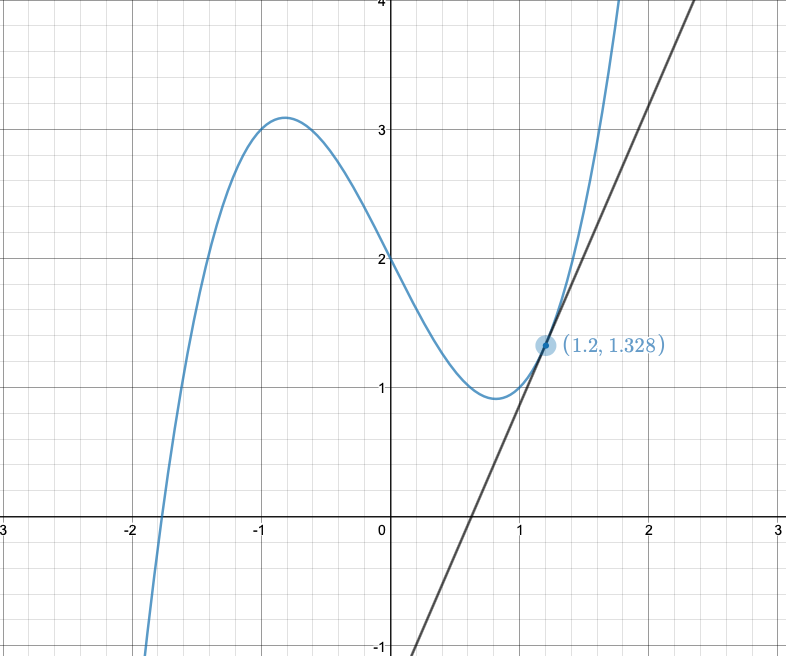
\includegraphics[width=\linewidth]{docs/newton-attempt.png}
  \caption{Tanget line of graph of $f(x)$}
  % \label{fig:boat1}
\end{figure}


\section*{Question 2} % Unnumbered section
The derivative of $sin(x)$ at $x = 2$ can be approximated using $\frac{1}{h}(sin(2 + h) - sin(2)$. Type
the following three lines in Matlab to create a figure of the error $ \mid cos(2) - \frac{1}{h}(sin(2+h) - sin(2)) \mid $
for various values of $h = 1, 10^{-1}, 10^{-2}, . . . , 10^{-20}$ \\

\noindent
(a) (2 pts.) Error is expected to decrease with $h$, as we observe on the right part of the plot. The left part of the plot however, shows that exactly the opposite occurs. Explain why the error increases with decreasing $h$ beyond a certain point $ (h \simeq 10^{-8}) $ . \\

\noindent
As you approach ($\simeq 10^{-8}$) the error is no longer improved by decreasing the step size, and the roundoff error begins to accumulate due to worse and worse approximations. I.e the truncation error is only diminished to the point at which accurate approximations can be made.\\

\begin{figure}[H]
  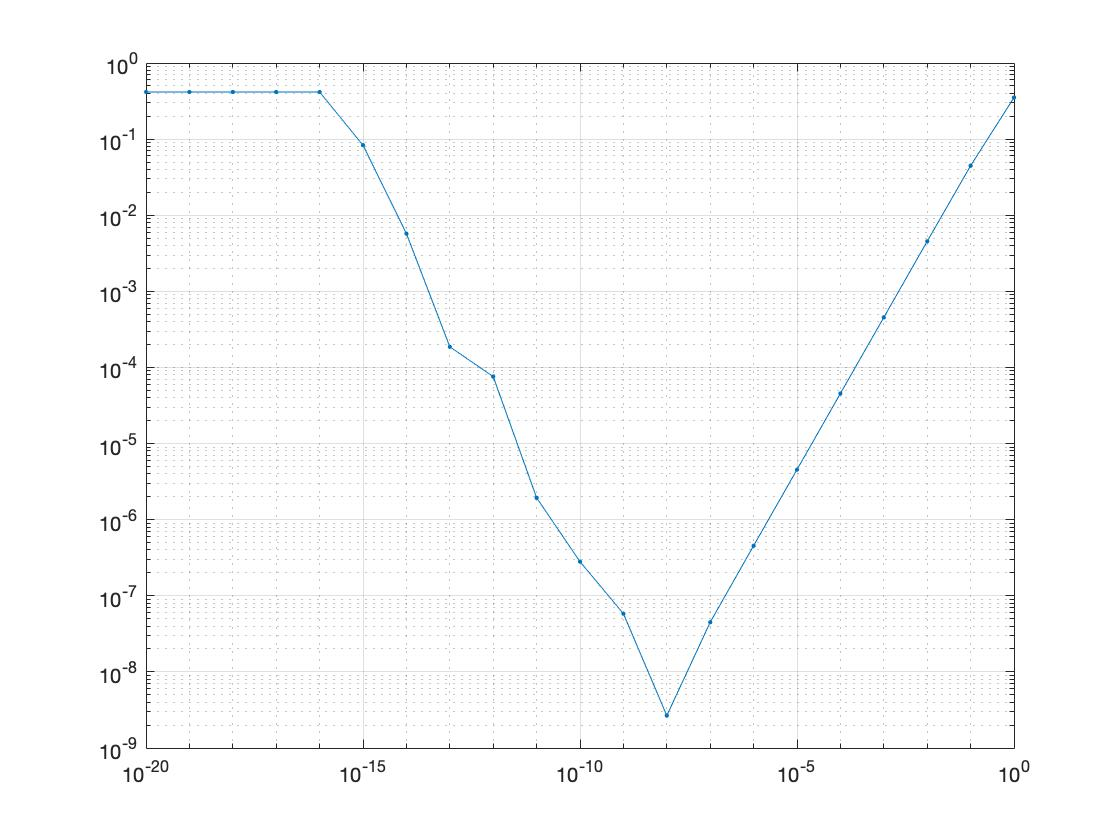
\includegraphics[width=\linewidth]{docs/error_calc.jpg}
  \caption{Tanget line of graph of $f(x)$}
  % \label{fig:boat1}
\end{figure}

\noindent
(b) (2pts.) Error appears to be exactly the same value $( \simeq 0.416147)$ for $h=10^{-16},10^{-17},10^{-18}, 10^{-19}, 10^{-20}$. Explain why. Where does this value come from? \\

\noindent
Because $ \epsilon_{mach} \simeq 10^{-16}$, therefore the function $ \mid cos(2) - \frac{1}{h}(sin(2+h) - sin(2)) \mid $ will yield the same approximation, and thus the same error.\\

\noindent
(c) (2 pts.) We know that this is a first order approximation to the first derivative. Since the figure shows how the error changes for various values of h, it is possible to estimate the order of this method using this figure. Verify that this is a first order method (or very close, it is an estimate after all) by using the figure. Feel free to print the figure and draw lines on it if it helps.\\

\noindent
The graph is linear which shows uniform change in Y, as X changes. Emphrically when $ h = 10^{-7}, \text{error} = 4.485 x 10^{-8}$ and $h = 10^{-8}, \text{error} = 4.547 x 10^{-7}$ so decreasing h by a factor of 10 decreases the error by $10x$ so this appoximation is first order.\\

\noindent
d) (2 pts.) Replace the second line (errors = ...) to use the fourth order approximation to the first derivative, which you derived in the previous assignment:

\begin{gather*}
  f^{\prime(x)} \simeq \frac{-f(x+2h) + 8f(x+h) - 8f(x-h) + f(x - 2h)}{12h} + \bigO(h^{4})
\end{gather*}\\

\noindent
The minimum error you can achieve with the previous method is between $10^{-8}$ and $10^{-9}$. What is the minimum error you can achieve change with this new method? Given that your computer’s precision is fixed, clearly explain the reason for the improvement in the minimum error.\\

\begin{figure}[H]
  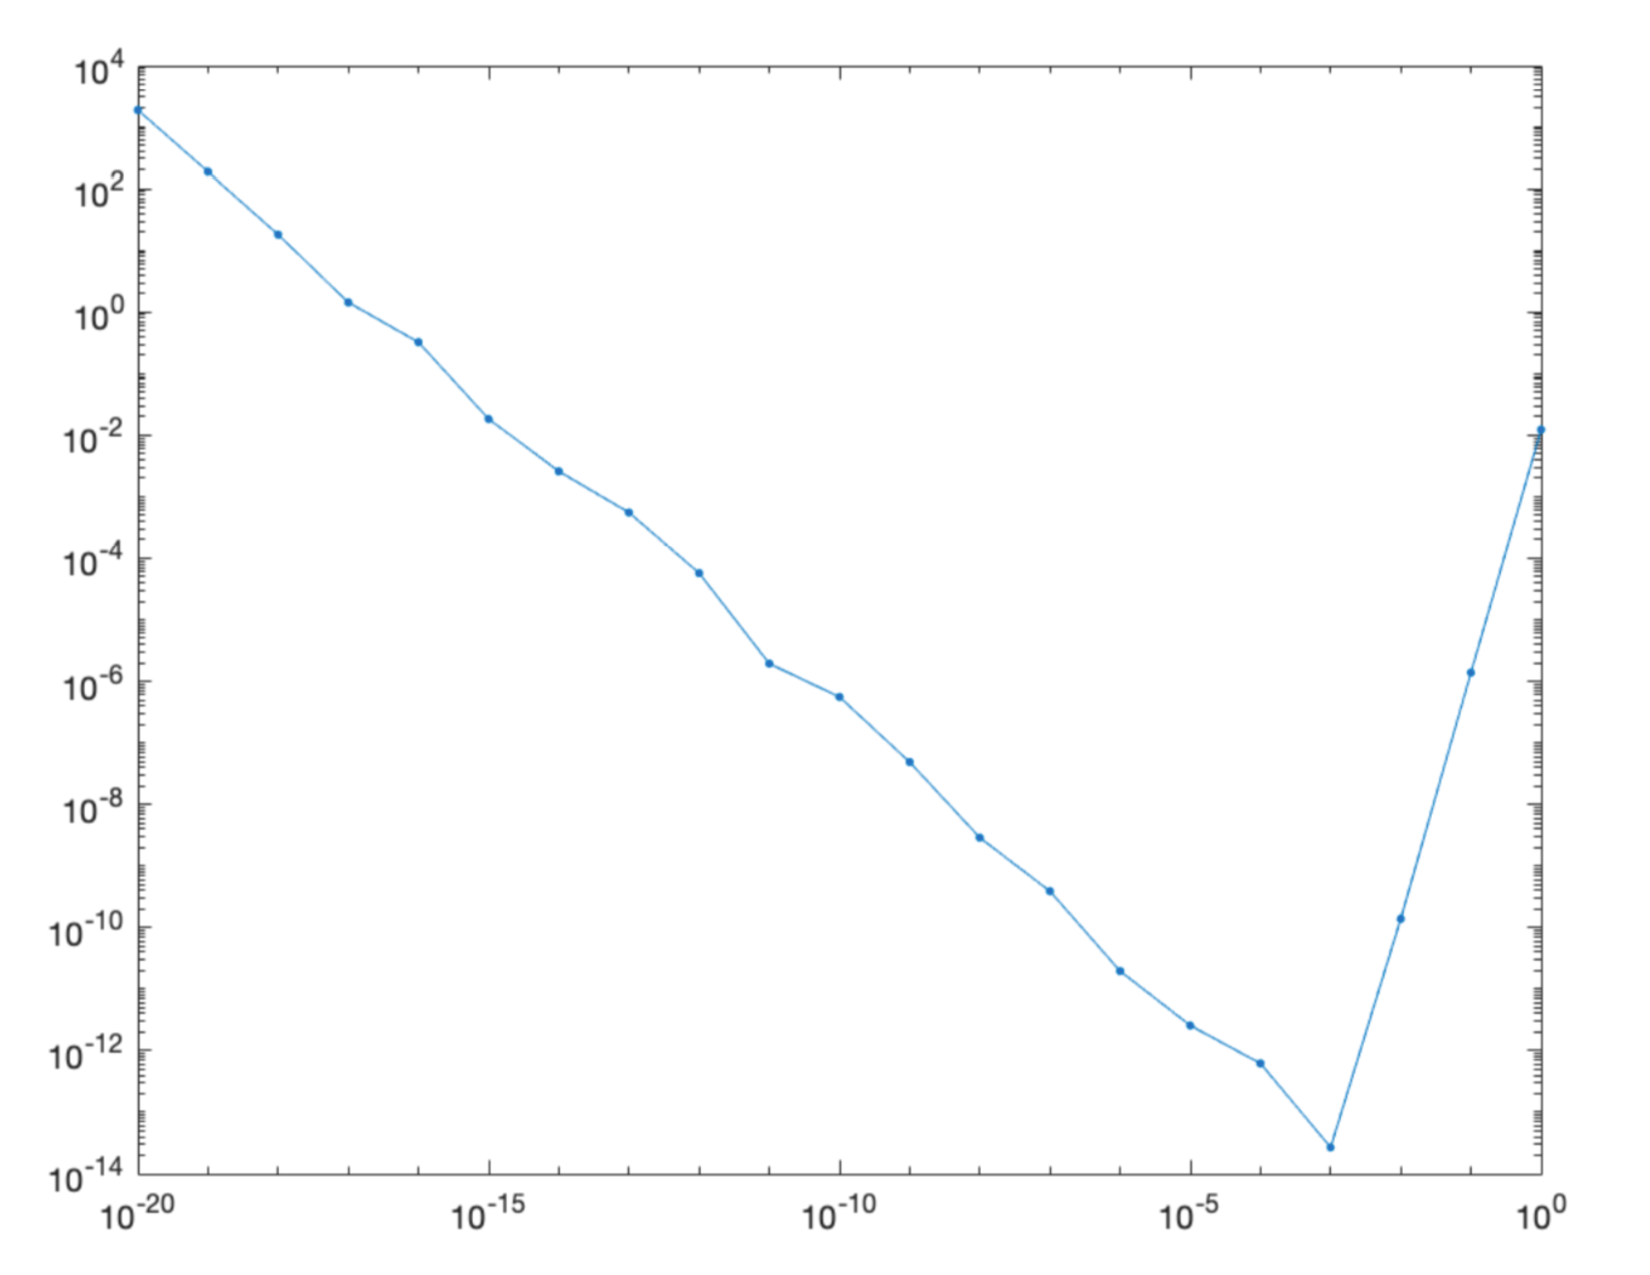
\includegraphics[width=\linewidth]{docs/error-graph.pdf}
  \caption{Fourth order error approximation}
  % \label{fig:boat1}
\end{figure}

\noindent
The new minimum error is $\simeq 10^{-14}$ the higher order method allows for better approximations as $h$ decreases, this extra precision allows the number to have higher resolution.\\

\noindent
(e) (2 pts.) Repeat part (c) for this new method.\\

\noindent
Decreaasing $h$ decrease by $10$ times the errors decrease $ \simeq 10^{4}$ times, so this system is $4_{th}$ order.

\section*{Question 3} % Unnumbered section
(15pts.)The concentration of pollutant bacteria $c(t)$ in a lake decreases according to the following expression (unit is $cfu/ml$):

\begin{gather*}
  c = 75e^{-1.5t} + 20e^{-0.075t}
\end{gather*}

\noindent
We’ll use various methods to determine the time required for the bacteria concentration to be reduced to a safe level of $15 cf u/ml$\\

\noindent
(5 pts.) Write a Matlab code to solve this problem using Newton’s method with an initial guess of $t_{0} = 0$ and stopping criterion of 0.5\% approximate relative error. At each iteration, your code should print (i) iteration number, (ii) approximated value of t, and (iii) approximate relative error. Print your code and the output of your code, and include them in your solutions. Name your code as newton.m and submit a soft copy as an e-mail attachment with subject line “ENGR8103 HW3” to ml64719@uga.edu.\\

\lstinputlisting{/Users/allenspain/Desktop/hw3/newton.m}

\begin{verbatim}
OUTPUT:

----------------------------------------
(i) iteration: 1
(ii) approximated val: 0.701754
(iii)relative error: 1.000000
----------------------------------------
(i) iteration: 2
(ii) approximated val: 1.442789
(iii)relative error: 0.513613
----------------------------------------
(i) iteration: 3
(ii) approximated val: 2.253249
(iii)relative error: 0.359685
----------------------------------------
(i) iteration: 4
(ii) approximated val: 3.125065
(iii)relative error: 0.278975
----------------------------------------
(i) iteration: 5
(ii) approximated val: 3.805303
(iii)relative error: 0.178761
----------------------------------------
(i) iteration: 6
(ii) approximated val: 3.994018
(iii)relative error: 0.047249
----------------------------------------
\end{verbatim}


\lstinputlisting{/Users/allenspain/Desktop/hw3/secant.m}

\begin{verbatim}
OUTPUT:
i) iteration: 1
(ii) approximated val: 1.339801
(iii)relative error: 0.253620

----------------------------------------
(i) iteration: 2
(ii) approximated val: 1.603115
(iii)relative error: 0.164252
----------------------------------------
(i) iteration: 3
(ii) approximated val: 1.819303
(iii)relative error: 0.118830
----------------------------------------
(i) iteration: 4
(ii) approximated val: 2.003240
(iii)relative error: 0.091820
----------------------------------------
(i) iteration: 5
(ii) approximated val: 2.163499
(iii)relative error: 0.074074
----------------------------------------
(i) iteration: 6
(ii) approximated val: 2.305466
(iii)relative error: 0.061578
----------------------------------------
(i) iteration: 7
(ii) approximated val: 2.432752
(iii)relative error: 0.052322
----------------------------------------
(i) iteration: 8
(ii) approximated val: 2.547900
(iii)relative error: 0.045193
----------------------------------------
\end{verbatim}



\lstinputlisting{/Users/allenspain/Desktop/hw3/bisection.m}

\begin{verbatim}
OUTPUT

i) iteration: 1
(ii) approximated val: 5.000000
(iii)relative error: 2.500000
----------------------------------------
(i) iteration: 2
(ii) approximated val: 2.500000
(iii)relative error: 1.250000
----------------------------------------
(i) iteration: 3
(ii) approximated val: 1.250000
(iii)relative error: 0.625000
----------------------------------------
(i) iteration: 4
(ii) approximated val: 1.875000
(iii)relative error: 0.312500
----------------------------------------
(i) iteration: 5
(ii) approximated val: 2.187500
(iii)relative error: 0.156250
----------------------------------------
(i) iteration: 6
(ii) approximated val: 2.343750
(iii)relative error: 0.078125
----------------------------------------
(i) iteration: 7
(ii) approximated val: 2.421875
(iii)relative error: 0.039062
----------------------------------------
\end{verbatim}


\section*{Question 4} % Unnumbered section
(7 pts.) Consider the following equation system:

\begin{gather*}
  x + y + z = 0 \\
  x^2 + y^2 = 5 \\
  x(x+y) = -1
\end{gather*}

To find a solution this nonlinear equation system, carry out the first two Newton iterations starting with $(x_{0}, y_{0}, z_{0}) = (1, 1, 1)$ to find $ (x_{1}, y_{1}, z_{1})$ and $(x_{2}, y_{2}, z_{2})$. Show all your work clearly. Feel free to use a calculator to find the inverse of the matrix.\\

\noindent
From Newton's method for section

\begin{gather*}
  X_{n+1} = X_{n} - \left[ \triangledown f(X_{n})\right]^{-1}f(X_{n}) \\
  \begin{bmatrix}
    \frac{\partial f(x,y,z)_{1}}{\partial x}& \frac{f(x,y,z)_{1}}{\partial y} & \frac{f(x,y,z)_{1}}{\partial z} \\\frac{\partial f(x,y,z)_{2}}{\partial x}  & \frac{\partial f(x,y,z)_{2}}{\partial y} & \frac{\partial f(x,y,z)_{2}}{\partial z} \\ \frac{\partial f(x,y,z)_{3}}{\partial x} & \frac{\partial f(x,y,z)_{3}}{\partial y} &\frac{\partial f(x,y,z)_{3}}{\partial z}
  \end{bmatrix} =
  \begin{bmatrix}
      1 & 1 & 1\\
      2x & 2x & 0 \\
      y + z & x & x
  \end{bmatrix}
\end{gather*}


Taking the inverse of the matrix:
\begin{gather*}
  \left[ \triangledown f(X_{n})\right]^{-1} =
  \begin{bmatrix}
      -\frac{x}{x+z-x} & 0 & \frac{1}{y+z-x}\\
      \frac{x^{2}}{y(y+z-x)} &\frac{1}{2y} & -\frac{x}{y(y+z-x)} \\
      \frac{y(y+z) - x^{2}}{y(y+z-x)} & -\frac{1}{2y} & -\frac{y-x}{y(y+z-x)}
    \end{bmatrix}
\end{gather*}

For the first iteration $(x_{0},y_{0}, z_{0}) = (1,1,1)$
\begin{gather*}
  \therefore X_{1} =
  \begin{bmatrix}
    1\\
    1\\
    1
  \end{bmatrix} -
  \begin{bmatrix}
    -1 & 0 & 1\\
    1 & 0.5 & -1 \\
    1 & -0.5 & 0
  \end{bmatrix}
  \begin{bmatrix}
    3 \\
    2 \\
    2
  \end{bmatrix} =
  \begin{bmatrix}
    1 \\ 1\\ 1
  \end{bmatrix} -
  \begin{bmatrix}
    -1 \\ 2 \\ 2
  \end{bmatrix} =
  \begin{bmatrix}
    2 \\ -1 \\ -1
  \end{bmatrix}\\
  \Rightarrow X_{1} = \begin{bmatrix} 2 \\ -1 \\ -1 \end{bmatrix}
\end{gather*}


For the second iteration $(x_{1},y_{1}, z_{1}) = (2,-1,-1)$
\begin{gather*}
  \therefore X_{1} =
  \begin{bmatrix}
    2\\
    -1\\
    -1
  \end{bmatrix} -
  \begin{bmatrix}
    0.5 & 0 & -0.25\\
    1 & -0.5 & -0.5 \\
    -0.5 & 0.5 & 0.75
  \end{bmatrix}
  \begin{bmatrix}
    0 \\
    5 \\
    -4
  \end{bmatrix} =
  \begin{bmatrix}
    2 \\ -1\\ -1
  \end{bmatrix} -
  \begin{bmatrix}
    1 \\ 0.5 \\ 0.5
  \end{bmatrix} =
  \begin{bmatrix}
    1 \\ -0.5 \\ -0.5
  \end{bmatrix}\\
  \Rightarrow X_{2} = \begin{bmatrix} 1 \\ -0.5 \\ -0.5 \end{bmatrix}
\end{gather*}






\end{document}
